This chapter is the final words that will conclude our analysis of Aparapi and JCuda.

\section{Aparapi or JCuda?}

For someone absolutely looking for the fastest solution, JCuda is more suitable than Aparapi. In our analysis, based on a matrix multiplication and a Levenshtein distance, JCuda is globally faster than Aparapi, with sometimes results more than 2 times faster than Aparapi. However, we observed one case on a particular string size for the Levenshtein distance computation where Aparapi was faster. So, even speaking of speed, Aparapi could be faster on particular cases. Globally, JCuda is faster but we couldn't test every cases on every computation types.

Speaking about ease of use, Aparapi wins the palm and is more suitable than JCuda. It requires less line of codes, has the advantage of being entirely usable in Java and doesn't need an CUDA environment, which is not always possible for someone not having an NVDIA GPU.

JCuda requires a kernel written in C, which could be either an advantage or a disadvantage. Someone already familiar with JCuda won't have any difficulties since the kernel whould be the same, but for someone not familiar with CUDA programming it will be more difficult to get started compared to Aparapi.

If keeping an absolute Java environment is a priority, Aparapi comes as the only possible solution. With Aparapi, everything is written in Java, providing a smooth development workflow and a clear code. It also gives the abilities of writing custom Java methods helper available from the kernel - which is not possible with JCuda.

\section{The answer}

Answering the question "should I use Aparapi od JCuda?" requires to know what are the needs and the development environment available. It maily requires to answer three questions :

\begin{enumerate}
  \item Do we have a CUDA or OpenCL environment?
  \item Do I want to keep the code simple and stay exclusively with Java?
  \item Am I focused on speed?
\end{enumerate}

The process to guide the choice of Aparapi or JCuda based on the previous questions is given by the flowchart in the figure \ref{fig: flow final choice}.

\begin{figure}[h]
\centering
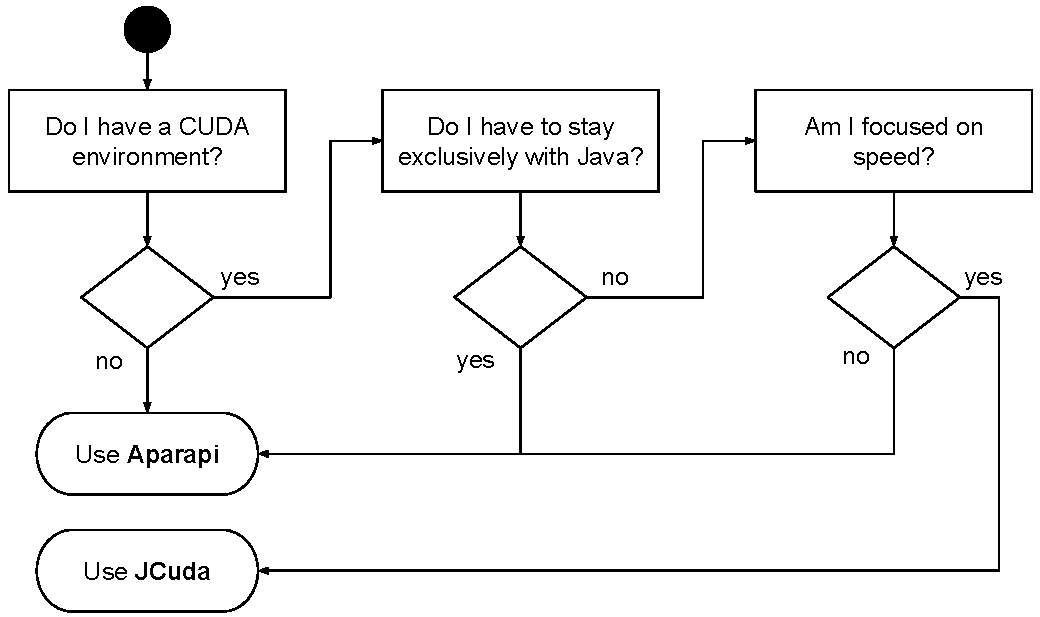
\includegraphics[width=1\textwidth]{final_flow}
\caption{Flowchart guiding the decision of using either Aparapi or JCuda}
\label{fig: flow final choice}
\end{figure}

However, this process may not be true on every cases, especially speaking of speed where Aparapi could be faster on some cases - and we obviously couldn't test every cases for every computation types. We are only saying that JCuda is globally faster, but there could be cases where it is not. The last question on the flow "Am I focused on speed?" could lead to JCuda even if the answer is "no" for someone who prefers using a CUDA based solution anyway. At this point of the flow, it is more a question of flavor. We tried, on the flow, to fit the most global use case and answer the question for, what we think, corresponds to the majority.

\section{Perspectives}

There are some points that could be expanded and leave some future perspectives. We are thinking of :

\begin{itemize}
  \item Testing more solutions
  \item Developping more benchmarks
  \item Increasing the measures' precisions
\end{itemize}

Aparapi and JCuda are of course not the only solutions that make GPU programming available from Java. In our pre-analysis (see table \ref{pre analysis}), we had 11 candidates and we only evaluated 2 of them. We chose the first 2 of them that seemed the most promising to us, but evaluating more of them according to our test battery could lead us to better solutions.

Our test battery only uses 2 benchmarks. Having more benchmarks would give us more specific measures about what solution is the best for what kind of computation and parameter. As we saw, JCuda is globally faster than Aparapi. But in special cases, Aparapi is faster. With more benchmarks we would perhaps discover more special cases where Aparapi is  faster, and then giving a more precise way to make a decision between Aparapi and JCuda.

Our benchmark only measures the rounded seconds spent. Hense, the sequential time and the speedup suffer from an uncertainty that could be important in some cases. The uncertainty in our measures is discussed in appendix \ref{uncertain}. The uncertainty could be much reduced by measuring the sequential time in milliseconds instead of rounded seconds.